\section{Artificial Bee Colony Algorithm}

The Artificial Bee Colony (ABC) algorithm is a nature-inspired, meta-heuristic
optimisation algorithm. It was introduced by Karaboga \cite{beecolony} and is
motivated by the behaviour of honey bees.

The model defines three components: employed bees, unemployed bees, and food
sources. Employed bees search for new food sources by looking in the
neighbourhood of other food sources they have memorised. They show the gathered
information to the unemployed onlooker bees which get recruited by a
probability dependent on the food source quality, called fitness. Employed bees
that are not able to improve the quality of their food source multiple times
(i.e. hit the abandonment limit) will become unemployed scout bees search for a
new food source randomly.

Since we are seeking to solve the Travelling Salesman Problem (TSP), each food
source is defined as a route of cities. Each city is defined by a x and a y
coordinate. In the TSP we aim to get the optimal order of cities, which leads
to a minimal travelling distance. We introduce problem specific knowledge to
the algorithm by defining its neighbourhood search. Based on the idea from Li
et al. \cite{beetsp}, we obtain the neighbour of a route by swapping the order
of some cities. Each city will get swapped with a certain probability, and it
will get swapped with a randomly chosen city. In this case, the fitness of a
food source is the distance of a route of cities.

\subsection{Experiments}

In this section, we compare our implementation of the Artificial Bee Colony
algorithm to the reference evolutionary algorithm on the TSP problem.

In \cref{tab:bee_vs_ea} and \cref{fig:bee_vs_ea} we see the ABC algorithm
performed slightly worse than the reference evolutionary algorithm. As the
standard deviations in \cref{tab:bee_vs_ea} show, the results of the ABC
algorithm where more stable when compared to the EA.

For our tests, we initialised 40 bees and optimise over 1000 iterations. We set
the randomisation factor $\alpha = 0.005$ and the abandonment limit to 200.
The two approaches are very comparable in terms of their run-time, although the
bee colony algorithm performs a higher number of evaluations over the same
amount of iterations.

\begin{figure}[h]
  \centering
  \begin{subfigure}{.5\textwidth}
    \centering
    \captionsetup{width=0.75\linewidth}
    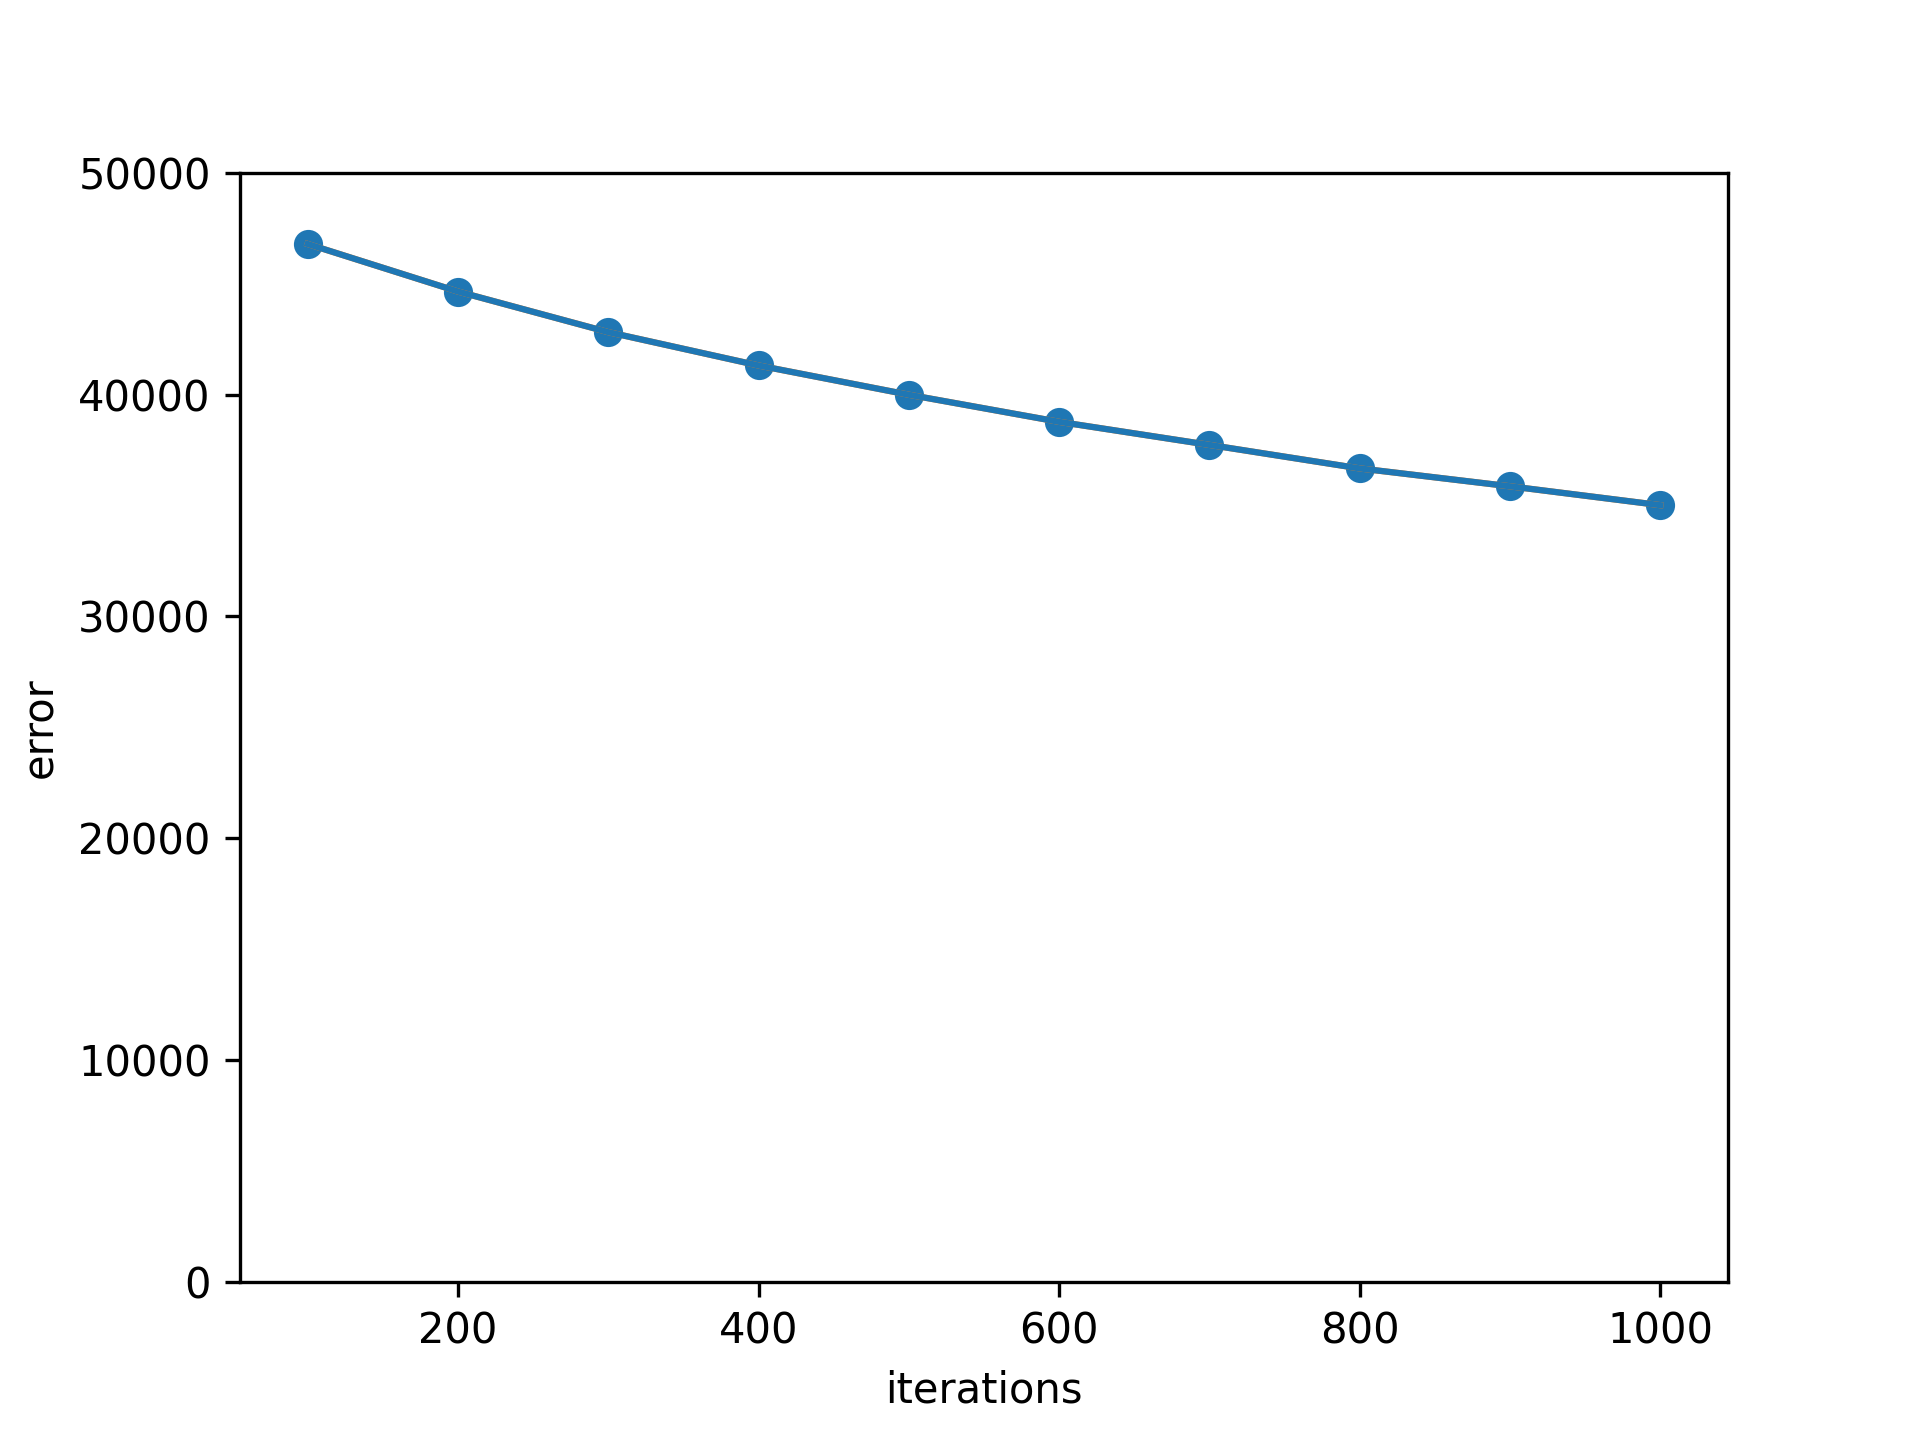
\includegraphics[width=0.75\linewidth]{assets/reference_tsp.png}
    \caption{Error over iterations using the reference evolutionary algorithm.}
    \label{fig:reference_tsp}
  \end{subfigure}%
  \begin{subfigure}{.4\textwidth}
    \centering
    \captionsetup{width=0.75\linewidth}
    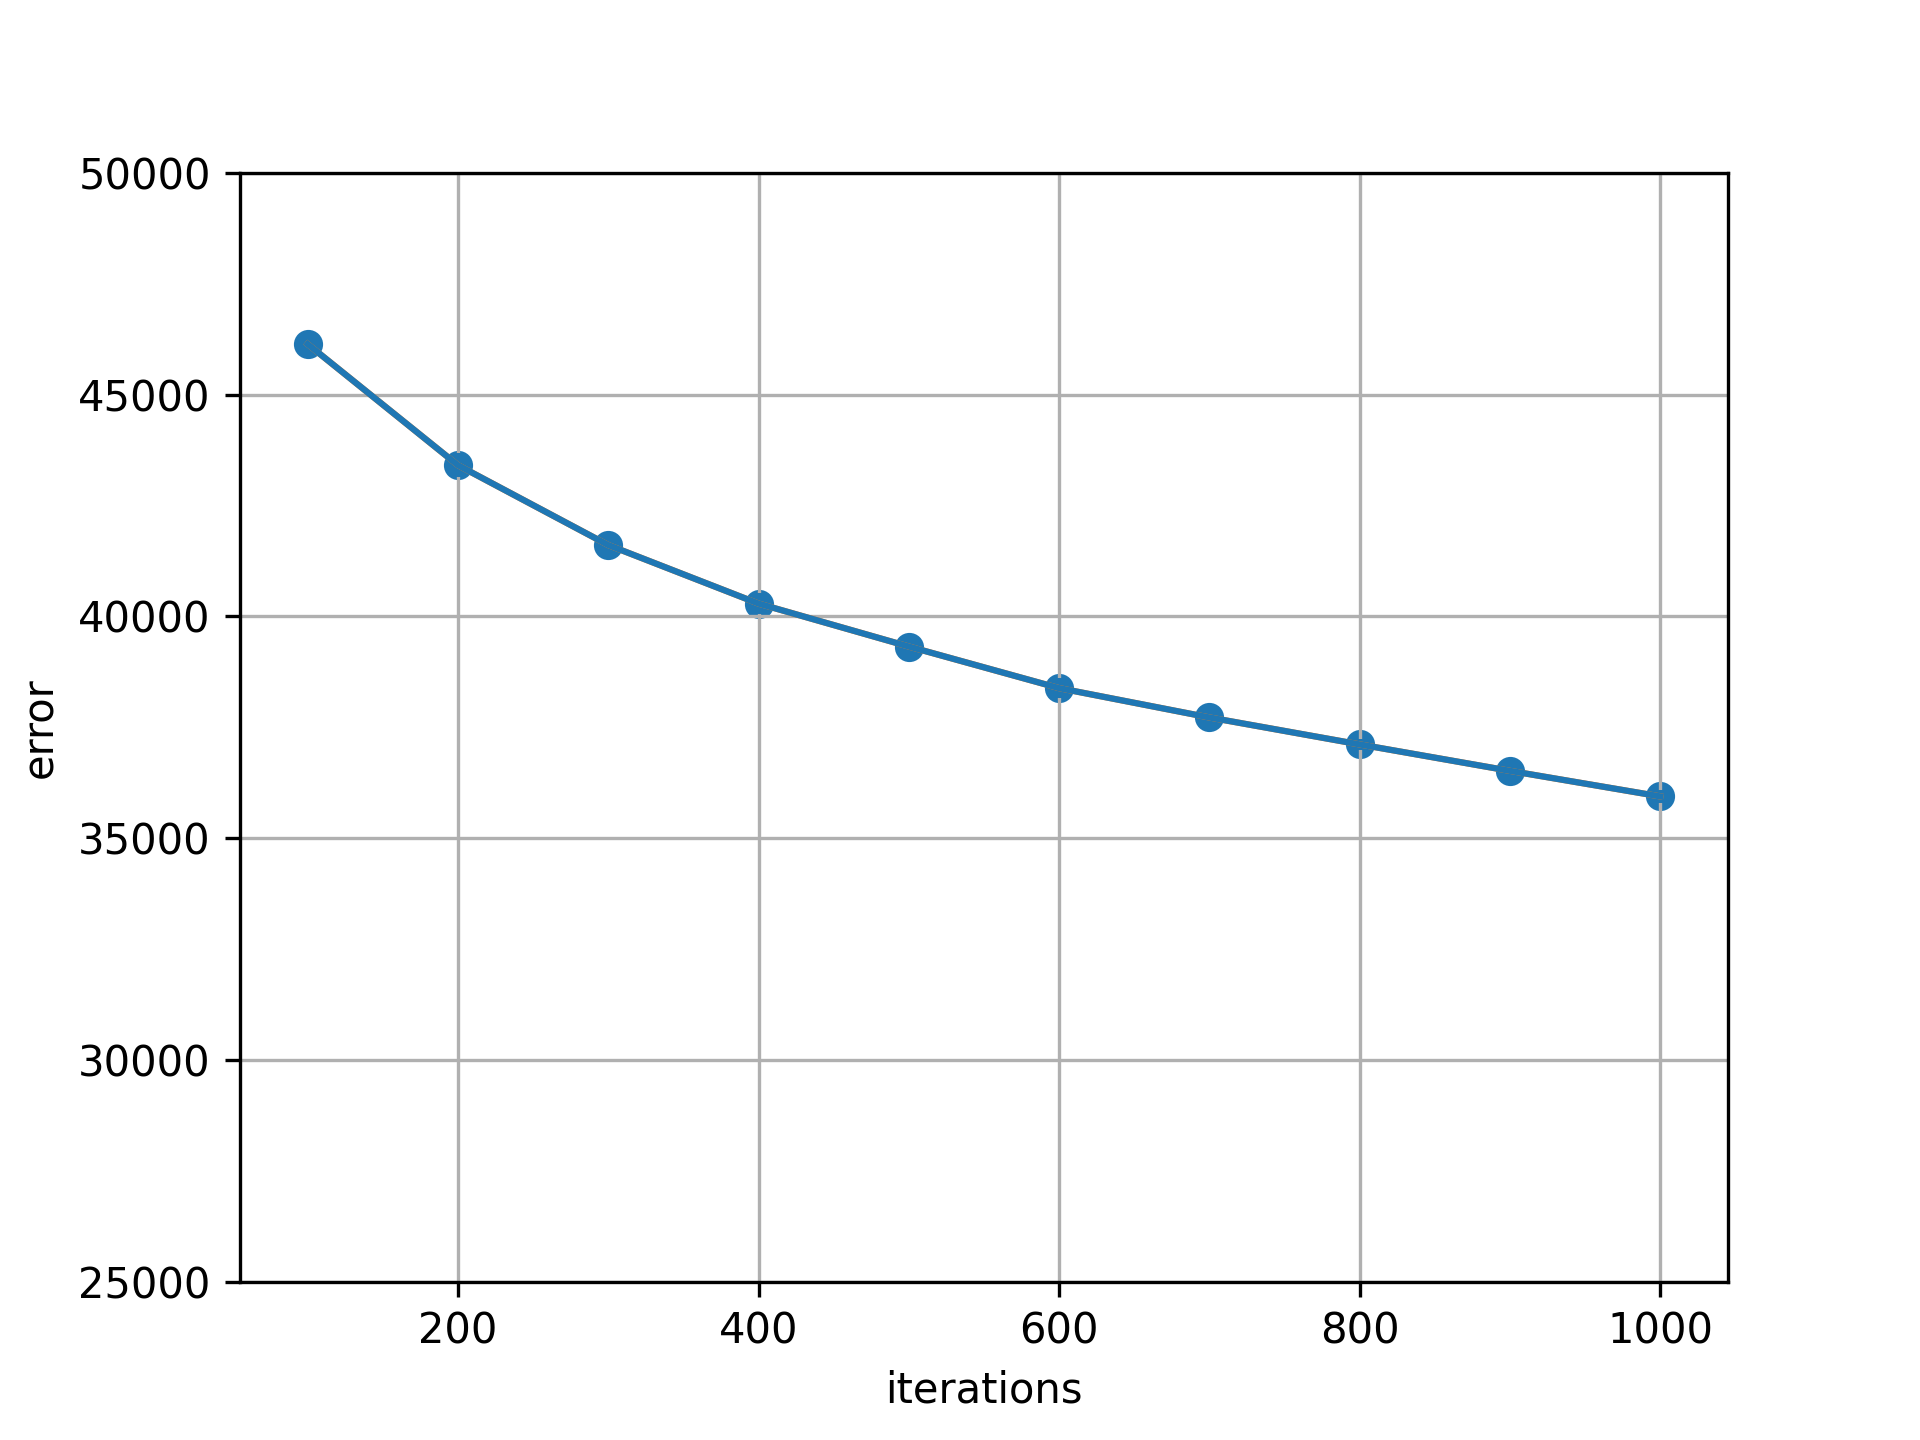
\includegraphics[width=0.75\linewidth]{assets/beecolony_tsp.png}
    \caption{Error over iterations using the bee colony algorithm.}
    \label{fig:becolony_tsp}
  \end{subfigure}
  \caption{Comparison of ABC and evolutionary algorithm on the TSP problem.}
  \label{fig:bee_vs_ea}
\end{figure}

\begin{table}[H]
  \centering
  \begin{tabular}{|l r r r|}
    \hline
    \textbf{Optimiser} & \textbf{Error ± Deviation} & \textbf{Evaluations} & \textbf{Run-time [s]} \\
    \hline
    Bee Colony Algorithm & 35939.18 ± 144.21 & 80040 & 2.93 \\
    Reference Evolutionary Algorithm & 35012.41 ± 482.07 & 25000 & 2.90 \\
    \hline
  \end{tabular}
  \caption{Minimal errors after the given number of evaluations produced by optimisers on the TSP problem. Results are averaged over 10 subsequent runs.}
  \label{tab:bee_vs_ea}
\end{table}
